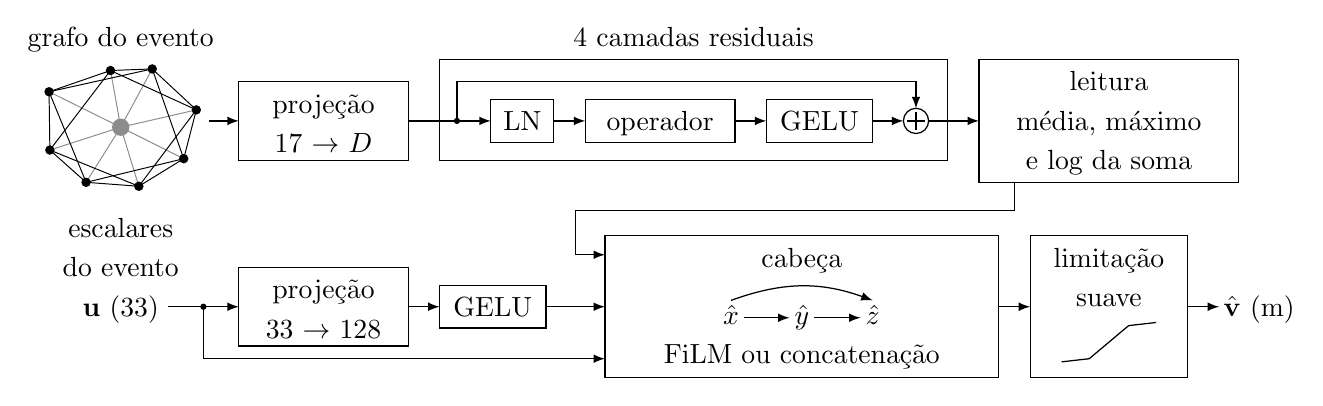
\begin{tikzpicture}[
  x=1cm, y=1cm,
  line width=0.45pt,
  flow/.style={-latex, line width=0.45pt},
  knn/.style={line width=0.35pt},
  spoke/.style={line width=0.35pt, draw=black!45},
  channel/.style={circle, fill=black, inner sep=0pt, minimum size=1.2mm},
  globalnode/.style={circle, fill=black!45, inner sep=0pt, minimum size=2.2mm},
  branch/.style={circle, fill=black, inner sep=0pt, minimum size=0.8mm},
  txt/.style={inner sep=0pt, anchor=base},
  dag/.style={inner sep=1.6pt, execute at begin node={\vphantom{$\hat{x}\hat{y}\hat{z}$}}}
]
\def\arqrowa{3.28}
\def\arqrowb{0.92}
\def\arqgap{2.14}
\def\arqtop{4.22}

\coordinate (g)  at (1.45, 3.20);
\coordinate (c0) at (2.41, 3.42);
\coordinate (c1) at (1.85, 3.94);
\coordinate (c2) at (1.32, 3.92);
\coordinate (c3) at (0.54, 3.65);
\coordinate (c4) at (0.55, 2.91);
\coordinate (c5) at (1.01, 2.50);
\coordinate (c6) at (1.68, 2.45);
\coordinate (c7) at (2.25, 2.80);

\foreach \i in {0,...,7} {\draw[spoke] (g) -- (c\i);}
\foreach \i/\j in {0/1,1/2,2/3,3/4,4/5,5/6,6/7,7/0,0/2,1/3,2/4,3/5,4/6,5/7,6/0,7/1} {\draw[knn] (c\i) -- (c\j);}
\foreach \i in {0,...,7} {\node[channel] at (c\i) {};}
\node[globalnode] at (g) {};
\node[txt] at (1.45, \arqtop) {grafo do evento};

\draw[flow] (2.57, \arqrowa) -- (2.95, \arqrowa);
\draw (2.95, \arqrowa-0.50) rectangle (5.10, \arqrowa+0.50);
\node[txt] at (4.025, \arqrowa+0.10) {projeção};
\node[txt] at (4.025, \arqrowa-0.40) {\num{17} $\to$ $D$};

\draw (5.50, \arqrowa-0.50) rectangle (11.95, \arqrowa+0.78);
\node[txt] at (8.725, \arqtop) {\num{4} camadas residuais};
\draw[flow] (5.10, \arqrowa) -- (6.15, \arqrowa);
\node[branch] at (5.72, \arqrowa) {};
\draw[flow] (5.72, \arqrowa) -- (5.72, \arqrowa+0.50) -- (11.55, \arqrowa+0.50) -- (11.55, \arqrowa+0.16);
\draw (6.15, \arqrowa-0.27) rectangle (6.95, \arqrowa+0.27);
\node[txt] at (6.55, \arqrowa-0.12) {LN};
\draw[flow] (6.95, \arqrowa) -- (7.35, \arqrowa);
\draw (7.35, \arqrowa-0.27) rectangle (9.25, \arqrowa+0.27);
\node[txt] at (8.30, \arqrowa-0.12) {operador};
\draw[flow] (9.25, \arqrowa) -- (9.65, \arqrowa);
\draw (9.65, \arqrowa-0.27) rectangle (11.00, \arqrowa+0.27);
\node[txt] at (10.325, \arqrowa-0.12) {GELU};
\draw[flow] (11.00, \arqrowa) -- (11.39, \arqrowa);
\draw (11.55, \arqrowa) circle (0.16);
\draw (11.44, \arqrowa) -- (11.66, \arqrowa);
\draw (11.55, \arqrowa-0.11) -- (11.55, \arqrowa+0.11);
\draw[flow] (11.71, \arqrowa) -- (12.35, \arqrowa);

\draw (12.35, \arqrowa-0.78) rectangle (15.65, \arqrowa+0.78);
\node[txt] at (14.00, \arqrowa+0.38) {leitura};
\node[txt] at (14.00, \arqrowa-0.12) {média, máximo};
\node[txt] at (14.00, \arqrowa-0.62) {e log da soma};

\draw[flow] (12.80, \arqrowa-0.78) -- (12.80, \arqgap) -- (7.225, \arqgap) -- (7.225, \arqrowb+0.66) -- (7.60, \arqrowb+0.66);

\node[txt] at (1.45, \arqrowb+0.88) {escalares};
\node[txt] at (1.45, \arqrowb+0.38) {do evento};
\node[txt] at (1.45, \arqrowb-0.12) {$\mathbf{u}$ (\num{33})};
\draw[flow] (2.05, \arqrowb) -- (2.95, \arqrowb);
\node[branch] at (2.50, \arqrowb) {};
\draw[flow] (2.50, \arqrowb) -- (2.50, \arqrowb-0.66) -- (7.60, \arqrowb-0.66);
\draw (2.95, \arqrowb-0.50) rectangle (5.10, \arqrowb+0.50);
\node[txt] at (4.025, \arqrowb+0.10) {projeção};
\node[txt] at (4.025, \arqrowb-0.40) {\num{33} $\to$ \num{128}};
\draw[flow] (5.10, \arqrowb) -- (5.50, \arqrowb);
\draw (5.50, \arqrowb-0.27) rectangle (6.85, \arqrowb+0.27);
\node[txt] at (6.175, \arqrowb-0.12) {GELU};
\draw[flow] (6.85, \arqrowb) -- (7.60, \arqrowb);

\draw (7.60, \arqrowb-0.90) rectangle (12.60, \arqrowb+0.90);
\node[txt] at (10.10, \arqrowb+0.50) {cabeça};
\node[dag] (xh) at (9.20, \arqrowb-0.14) {$\hat{x}$};
\node[dag] (yh) at (10.10, \arqrowb-0.14) {$\hat{y}$};
\node[dag] (zh) at (11.00, \arqrowb-0.14) {$\hat{z}$};
\draw[flow] (xh) -- (yh);
\draw[flow] (yh) -- (zh);
\draw[flow] (xh.north) to[bend left=20] (zh.north);
\node[txt] at (10.10, \arqrowb-0.72) {FiLM ou concatenação};
\draw[flow] (12.60, \arqrowb) -- (13.00, \arqrowb);

\draw (13.00, \arqrowb-0.90) rectangle (15.00, \arqrowb+0.90);
\node[txt] at (14.00, \arqrowb+0.50) {limitação};
\node[txt] at (14.00, \arqrowb) {suave};
\draw (13.40, \arqrowb-0.70) -- (13.75, \arqrowb-0.66) -- (14.25, \arqrowb-0.24) -- (14.60, \arqrowb-0.20);
\draw[flow] (15.00, \arqrowb) -- (15.40, \arqrowb);
\node[txt, anchor=base west] at (15.45, \arqrowb-0.12) {$\hat{\mathbf{v}}$ (m)};
\end{tikzpicture}\relax
